\documentclass[11pt, letterpaper, titlepage]{article}
\usepackage[utf8]{inputenc}
\usepackage{hyperref}
\hypersetup{pdfborder=0 0 0}
\usepackage{amsmath}
\usepackage{amssymb}
\usepackage{geometry}
\usepackage[none]{hyphenat}
\usepackage{xcolor}
\usepackage{cite}
\usepackage{lipsum}
\usepackage{physics}
\usepackage{textgreek}
\usepackage{unicode-math}
\usepackage{subfigure}
\usepackage{graphicx}
\usepackage{textgreek}
\geometry{
 a4paper,
 left=25mm,%left=20mm,
 right=25mm,%right=20mm,
 bottom=25mm, %bottom=20mm,
 top=25mm,%top=20mm,
 }


%%%%%%%% PORTADA
\title{
 \textbf{\LARGE UNIVERSITY OF OSLO} \\
\vspace{37mm}
\textbf{\Large Project 1}\\
\vspace{7mm}
\Large FYS5419 – Project1
\vspace{25mm}
} 

\author{\Large Hishem Kløvnes }


        % \vspace{45mm}
        

\date{\Large 7 October 2024} % Deadline



\begin{document}
\maketitle
% \tableofcontents
\newpage




\section{a)}
In this project, there are a few matrices that will be used repetedly. So before doing anything, I will formulate them here first. 
The three Pauli matrices: 
\[
\begin{aligned}
σ_x &= \begin{pmatrix}  
        0 & 1 \\
        1 & 0
\end{pmatrix}\\
σ_y &= \begin{pmatrix}
        0 &-i\\
        i & 0
\end{pmatrix}\\
σ_z  &= \begin{pmatrix}
      1 & 0\\
      0 &-1  
\end{pmatrix}
\end{aligned}
\] 
The Hadamard and Phase gate
\[
\begin{aligned}
        H &= \frac{1}{\sqrt{2}} \begin{pmatrix}
                1&1\\1&-1
        \end{pmatrix}\\
        S &= \begin{pmatrix}
                1&0\\0&i
        \end{pmatrix},
\end{aligned}
\]
and the CNOT gate
\[
\begin{aligned}
        CNOT &= \begin{pmatrix}
                1&0&0&0\\
                0&1&0&0\\
                0&0&0&1\\
                0&0&1&0
        \end{pmatrix}
\end{aligned}
\]

In this part of the project, the goal was to take a one qubit basis, apply the right gates to it - creating a Bell state - and then measure the state. The states we use are simply \(\ket{0} = [1,0]\) and \(\ket{1} = [0,1]\). The Bell state is given by
\[
\begin{aligned}
        \ket{\Phi^+} &= \frac{1}{\sqrt{2}}(\ket{00} + \ket{11})\\
        \ket{\Phi^-} &= \frac{1}{\sqrt{2}}(\ket{00} - \ket{11})\\
        \ket{\Psi^+} &= \frac{1}{\sqrt{2}}(\ket{01} + \ket{10})\\
        \ket{\Psi^-} &= \frac{1}{\sqrt{2}}(\ket{01} - \ket{10})
\end{aligned}
\]
where $\ket{00}$ is the state where both qubits are in the state $\ket{0}$, and $\ket{11}$ is the state where both qubits are in the state $\ket{1}$. \newline
The first thing I did was to apply the Hadamard gate and the Phase gate to the one qubit basis to see what happens. 
\[
\begin{aligned}
H \ket{0} &= \frac{1}{\sqrt{2}}\begin{pmatrix}
        1&1\\1&-1
\end{pmatrix}
\begin{pmatrix}
  1\\0
\end{pmatrix} = \frac{1}{\sqrt{2}} \begin{pmatrix}
        1\\1
\end{pmatrix}\\
H \ket{1} &= \frac{1}{\sqrt{2}}\begin{pmatrix}
        1&1\\1&-1
\end{pmatrix}
\begin{pmatrix}
        0\\1
\end{pmatrix} = \frac{1}{\sqrt{2}}\begin{pmatrix}
        1\\-1
\end{pmatrix}\\
\end{aligned}
\] 
This means that after applying the Hadamard gate to the one-qubit basis, we get a pair of new states which are defined as superpositions of the original states. Here the new superpositioned states are almost identical. The only difference is the sign of the second state, which represents that the state points along \(-X\) axis on the bloch sphere, in contrast to the first state which points along the \(X\) axis. \newline
The next step was to apply the Phase gate to the one-qubit basis.
\[
\begin{aligned}
S \ket{0} &= \begin{pmatrix}
        1&0\\0&i
\end{pmatrix}
\begin{pmatrix}
        1\\0
\end{pmatrix} = \begin{pmatrix}
        1\\0
\end{pmatrix}\\
S \ket{1} &= \begin{pmatrix}
        1&0\\0&i
\end{pmatrix}
\begin{pmatrix}
        0\\1
\end{pmatrix} = \begin{pmatrix}
        0\\i
\end{pmatrix}
\end{aligned}
\]
This means that the Phase gate does not change the state of the qubit in the $\ket{0}$ state, but it changes the state of the qubit in the $\ket{1}$ state. The \(\ket{1}\) state still points to the south pole of the block sphere, but has acquired a phase factor of \(i\). \newline
The next step was to define Bell states. To do this, I first defined them explicitly, and then I created the Bell states by applying the right gates to each state. As I mentioned earlier there are four Bell states, and to create them I applied the CNOT and Hadamard gates to different tensor products of the one-qubit basis.
\[
\begin{aligned}
CNOT &⋅ (H \ket{0}) ⊗ \ket{0} = \frac{1}{\sqrt{2}} [1,0,0,1]\\
CNOT &⋅ (H \ket{1}) ⊗ \ket{0} = \frac{1}{\sqrt{2}} [0,1,1,0] \\
CNOT &⋅ (H \ket{0}) ⊗ \ket{1} = \frac{1}{\sqrt{2}} [1,0,0,-1] \\
CNOT &⋅ (H \ket{1}) ⊗ \ket{1} = \frac{1}{\sqrt{2}} [0,1,-1,0]
\end{aligned}
\]
I double checked these states with the definition of the Bell states, and they are correct. The next step was to apply the Hadamard gate and thereafter the CNOT gate to the Bell states. Let's take the first Bell state as an example. 
\[
\begin{aligned}
CNOT &⋅ (H ⊗ I) \ket{\Phi^+} = \\
CNOT &⋅ \frac{1}{\sqrt{2}} \begin{pmatrix}
        1&1\\1-1
\end{pmatrix} ⊗ \begin{pmatrix}
        1&0\\0&1
\end{pmatrix} \ket{\Phi^+} =\\
CNOT &⋅ \frac{1}{\sqrt{2}} \begin{pmatrix}
        1&0&1&0\\0&1&0&1\\1&0&-1&0\\0&1&0&-1
\end{pmatrix} \ket{\Phi^+} =\\
CNOT &⋅ \frac{1}{2} \begin{pmatrix}
        1\\0\\0\\-1 
\end{pmatrix} = \frac{1}{2} \begin{pmatrix}
        1&0&0&0\\0&1&0&0\\0&0&0&1\\0&0&1&0
\end{pmatrix} \begin{pmatrix}
        1\\1\\1\\-1
\end{pmatrix} = \frac{1}{2} \begin{pmatrix}
        1\\1\\-1\\1
\end{pmatrix}
\end{aligned}
\]
When repeating this process for all our Bell states, we notice that all of them are superpositions of all states: \(\ket{00}, \ket{01}, \ket{10}, \ket{11}\). This means that it does not matter which of the modified Bell states we use to measure, because the outcome should be the same. \newline
\begin{figure}
        \begin{center}
                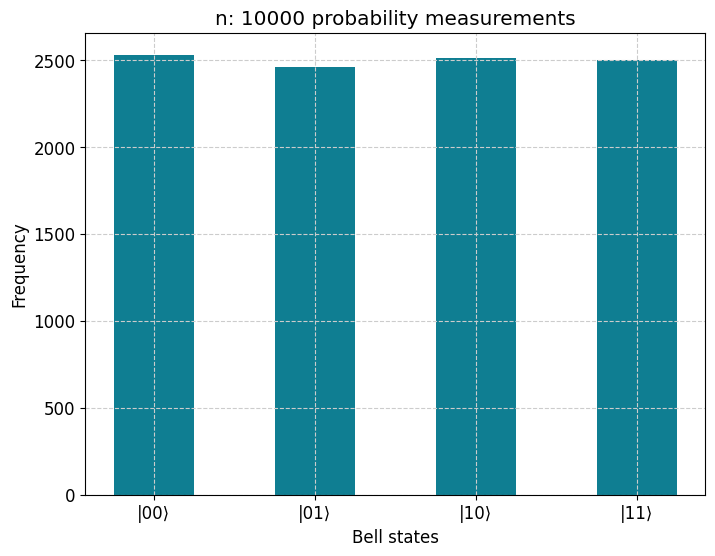
\includegraphics[scale=0.3]{BellMeasurement.png}
                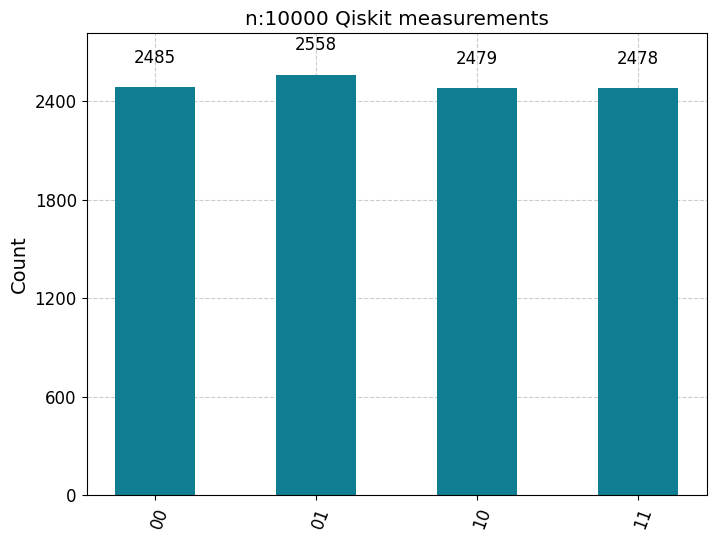
\includegraphics[scale=0.3]{BellMeasurementQiskit.png}       
        \end{center}
        \caption{The left figure shows the measurement of the Bell states using the method described above. The right figure shows the measurement of the Bell states using Qiskit.}
        \label{fig:BellMeasurement}
\end{figure}
In \ref{fig:BellMeasurement} Ihave compared the measurement of the Bell states using the method described above with the measurement of the Bell states using Qiskit. I did \(n=10000\) measurement on both methods, and the results are practically identical, which is what we would expect. For a system like this, we would expect the results to be around 25\% for each state. If we were to do even more measurements, \(n = 100000,1000000\cdots   \) we would expect the results to be even closer to 25\% for each state. \newline


\section{b)}
For this part of the problem, we have the same one-qubit basis as in the previous problem. Now we have a Hamiltonian \(H = H_0 + λH_I\), where
\[
H_0 = \mathcal{E} I + Ω σ_z, \quad \mathcal{E} = \frac{E_{1} + E_2}{2}, \quad Ω = \frac{E_1 - E_2}{2}
\]
and 
\[
H_I = cI + ω_zσ_z + ω_xσ_x
\]
where \(
c = (V_{11}+V_{22})/2, \quad ω_z = (V_{11}-V_{22})/2, \quad ω_x = V_{12}=V_{21}
\). We have a set of given values for our parameters:
\(E_1=0, E_2=4, V_{11}=V_{-22}=3, V_{12} = V_{21}=0.2\). \newline
In this section we want to find the eigenvalues of the Hamiltonian when acted on the one-qubit basis, as a function of the parameter \(λ\). This was solved numerically. 
I computed the eigenvalues of the Hamiltonian as a function of \(λ\), as shown in \ref{fig:Eigvals}. At \(λ\) the energy levels of \(\ket{0} \text{and} \ket{1}\) are separated by \(2Ω=4\). As \(λ\) increases, the interaction term \(H_I\) modifies the energy levels, causing them to converge. At \(λ=\frac{2}{3}\), the eigenvalues cross, which indicates degeneracy where the ground state and excited state have the same energy. When \(λ\) continues to increase, energy levels starts to separate again. \newline
The crossing is a level crossing, which occurs when the energy levels of the two states become degenerate. The physical interpretation of this result is that the system undergoes a transition at \(λ=\frac{2}{3}\), where the ground state and excited states exchanges. \newline
\begin{figure}
  \begin{center}
        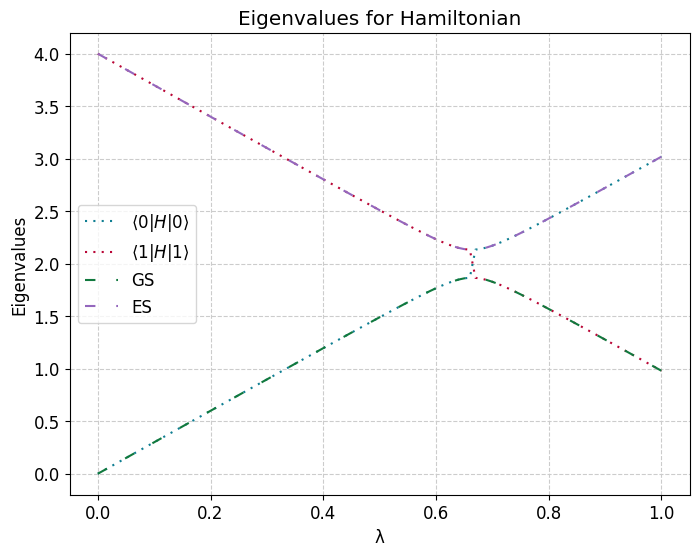
\includegraphics[scale=0.6]{Eigvals.png}
        \caption{The eigenvalues of the Hamiltonian as a function of the parameter \(λ\). ES represents the excited state, and GS represents the ground state.}
  \end{center}
  \label{fig:Eigvals}
\end{figure}\newpage
\section{c)}
In this section we want to attempt to implement the variational Quantum eigensolver (VQE) for the above Hamiltonian system.\newline
To do this I begun by defining the state  \(\ket{0}=[1,0]\). I also defined two rotation matrices \(R_x(θ)\) and \(R_y(ϕ)\), which are given by
\[
\begin{aligned}
R_x(θ) &= \cos(\frac{θ}{2})⋅ I - i \sin(\frac{θ}{2})⋅ σ_x\\
R_y(ϕ) &= \cos(\frac{ϕ}{2})⋅ I - i \sin(\frac{ϕ}{2})⋅ σ_y
\end{aligned}
\]
where \(θ\) and \(ϕ\) are the angles of rotation around the x and y axis, respectively, and \(I\) is the identity matrix. \newline
The process of the VQE method is to first prepare the state \(\ket{0}\), then apply the rotation matrices \(R_x(θ)\) and \(R_y(ϕ)\) to the state, with some arbitrary angles \(θ\) and \(ϕ\). After this, we measure the expectation value of the Hamiltonian, which is given by
\[
\begin{aligned}
\expval{H} &= \bra{\psi} H \ket{\psi} = \bra{\psi} H_0 \ket{\psi} + λ \bra{\psi} H_I \ket{\psi}
\end{aligned}
\]
where \(\ket{\psi}\) is the state after applying the rotation matrices. To find the optimal parameters for the rotation matrices, I used a gradient descent method, which is a method that minimizes a function by iteratively moving in the direction of the negative gradient. The gradient is calculated by 
\[
\begin{aligned}
        ∂ θ &= \pdv{\expval{H}}{θ},\\  ∂ ϕ &= \pdv{\expval{H}}{ϕ}
\end{aligned}
\]
And the parameters are updated by
\[
\begin{aligned}
        θ_{new} &= θ_{old} - \eta ∂ θ,\\ ϕ_{new} &= ϕ_{old} - \eta ∂ ϕ
\end{aligned}
\]
where \(η\) is the learning rate. This method was performed a number of times for each \(λ\), to find the optimal parameters.\newline
\begin{figure}
        \begin{center}
                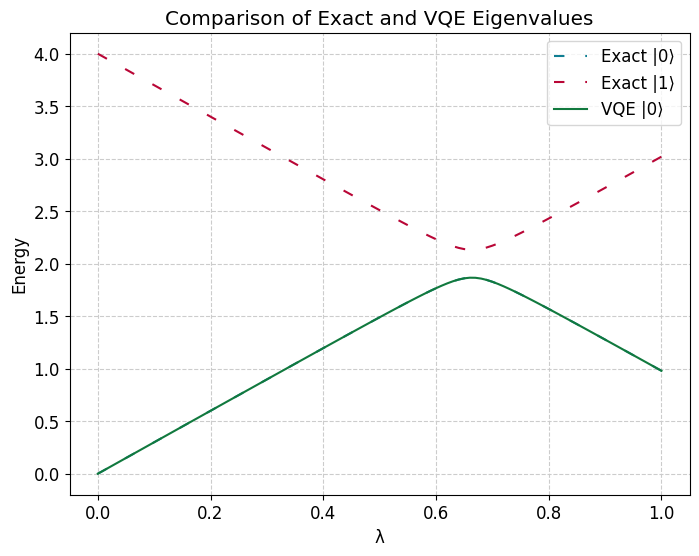
\includegraphics[scale=0.6]{VQE.png}
        \end{center}
        \caption{The figure shows a plot of the expectation value of the Hamiltonian as a function of the parameter \(λ\). The plot shows that the VQE method aligned perfectly with the ground state energy of the Hamiltonian.}
        \label{fig:VQE}
\end{figure}\newpage
In figure \ref{fig:VQE} I have plotted the expectation value of the Hamiltonian as a function of the parameter \(λ\). The plot shows that the VQE method aligned perfectly with the ground state energy of the Hamiltonian. Meaning that the VQE method was successful in finding the ground state energy of the Hamiltonian. The method of using gradient descent seemed to be a very effective and accurate method for the VQE of this simple system. \newline

\section{d)}
In this section we expand to a two-qubit system, where our many-bodu computational basis is given by \(\ket{00}, \ket{01}, \ket{10}, \ket{11}\), defined as:
\[
\begin{aligned}
\ket{00} &= \ket{0}_A ⊗ \ket{0}_B = [1\quad 0\quad 0\quad 0]^T \\
\ket{01} &= \ket{0}_A ⊗ \ket{1}_B = [0\quad 1\quad 0\quad 0]^T \\
\ket{10} &= \ket{1}_A ⊗ \ket{0}_B = [0\quad 0\quad 1\quad 0]^T \\
\ket{11} &= \ket{1}_A ⊗ \ket{1}_B = [0\quad 0\quad 0\quad 1]^T
\end{aligned}
\]
These basis states also define the eigenstates of the non-interacting Hamiltonian:
\[
\begin{aligned}
        H_0 \ket{00} &= ϵ_{00} \ket{00} \\
        H_0 \ket{10} &= ϵ_{10} \ket{10} \\
        H_0 \ket{01} &= ϵ_{01} \ket{01} \\
        H_0 \ket{11} &= ϵ_{11} \ket{11}
\end{aligned}
\]
And the interacting part of the Hamiltonian is given by
\[
H_I = H_x σ_x⊗ σ_x + H_z σ_z⊗ σ_z
\]
Thus our Hamiltonian matrix is given by
\[
\begin{pmatrix}
  ϵ_{00} + λ H_z &0&0&λH_x\\
  0&ϵ_{10} - λH_z & λH_x&0\\
  0&λH_x&ϵ_{01} - λH_z&0\\
  λH_x&0&0&ϵ_{11} + λ H_z
\end{pmatrix}
\]
To find the energy eigenvalues we have a set of parameters \(H_x=2.0,H_z=3.0,ϵ_{00}=0.0,ϵ_{10}=2.5,ϵ_{01}=6.5,ϵ_{11}=7.0\). I found the eigenvalues to this Hamiltonian by diagonalizing the matrix.
\begin{figure}
        \begin{center}
                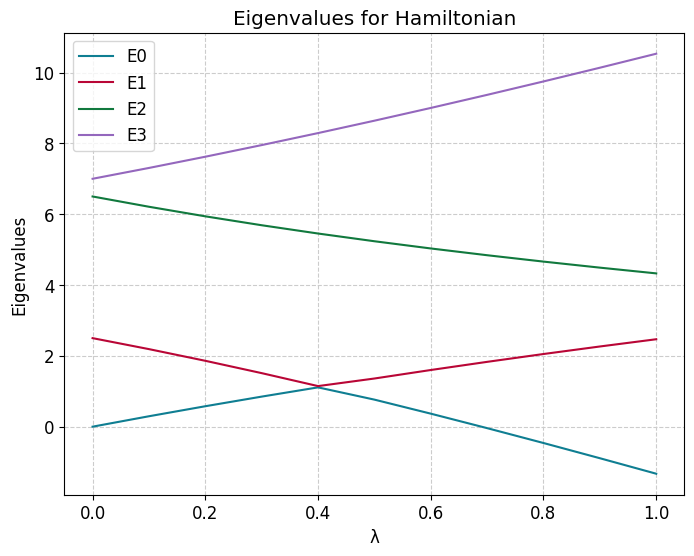
\includegraphics[scale=0.6]{Eigvals2q.png}
        \end{center}

        \caption{The figure shows the eigenvalues of the Hamiltonian as a function of the parameter \(λ\).}
        \label{fig:Eigvals2qubit}
\end{figure}\newpage
In figure \ref{fig:Eigvals2qubit} we see the energy eigenvalues of the Hamiltonian, as a function of the interaction parameter \(λ\). At \(λ=0.4\) we can, as in section b, see a level crossing where the ground state and excited state exchange. This shows how entanglement can be created in a system, by the Hamiltonian itself, due to the strength of the interaction. \newline
The next step is to calculate the von Neumann entropy of the same system. This is done by first defining the density matrix of the lowest energy eigenstate. 
\[
ρ_0 = (α_{00} \ket{00} \bra{00} + α_{10} \ket{10} \bra{10} + α_{01} \ket{01} \bra{01} + α_{11} \ket{11} \bra{11})
\]
We can then denfine the density matrices for the subsets \(A\) and \(B\), which are given by
\[
\begin{aligned}
ρ_A &= \text{Tr}_B(ρ_0) = \bra{0} ρ_0 \ket{0}_B +  \bra{1} ρ_0 \ket{1}_B\\
ρ_B &= \text{Tr}_A(ρ_0) = \bra{0} ρ_0 \ket{0}_A +  \bra{1} ρ_0 \ket{1}_A
\end{aligned}
\]
To find the von Neumann entropy, we will use the formula:
\[
S(A,B) = -\text{Tr}(ρ_{A,B}\log_2(ρ_{A,B}))
\]
\begin{figure}
        \begin{center}
                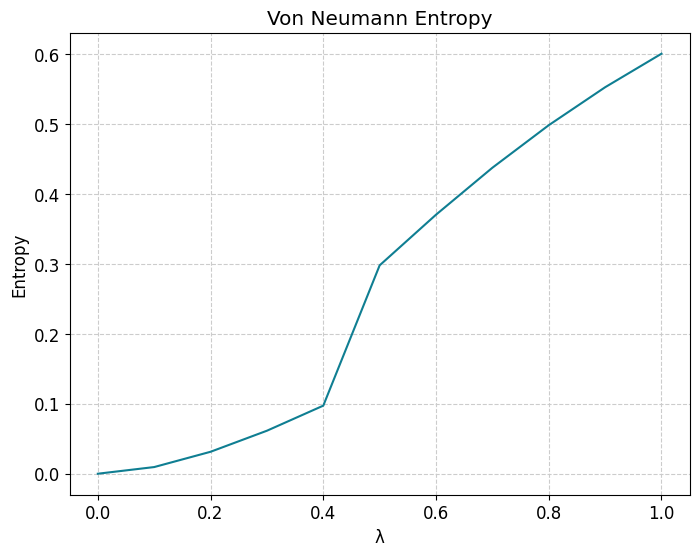
\includegraphics[scale=0.6]{VonNeumann.png}
        \end{center}
        \caption{The figure shows the von Neumann entropy of the system as a function of the parameter \(λ\).}
        \label{fig:VonNeumann}
\end{figure}
The results for this are shown in \ref{fig:VonNeumann}. The von Neumann entropy of the system is zero when the interaction parameter \(λ\) is zero, indicating no entanglement. As the interaction parameter increases, the von Neumann entropy increases, which is also what we would expect. The von Neumann entropy is a measure of the entanglement in the system, and the results show that the entanglement increases as the interaction parameter increases. At \(λ=0.4\) we can see a jump in the entropy, due to the sudden entanglement of the ground state and the first excited state. This can be compared with \(λ=0.4\) in \ref{fig:Eigvals2qubit}, where we can see the eigenvalues of the ground state and the first excited state cross. \newline


\section{e)}
In this section we will use the VQE method to approximate the ground state ennergy eigenvalues, for a range of \(λ\) values. This is done for the 2-qubit system, with the above hamiltonian and the same parameter values. This was done almost the same way as with the 1-qubit system, but with a few modifications. The state \(\ket{00}\) was defined as the initial state. The rotation matrices are the same ones I used in c), but I applied each of them twice, once for each qubit. The state was defined as
\[
\ket{\psi} = CNOT ⋅ ( R_x(θ_1) ⊗ R_x(θ_2)) ⋅  (R_y(ϕ_1) ⊗ R_y(ϕ_2) )\ket{00}
\]
\begin{figure}[h]
        \begin{center}
                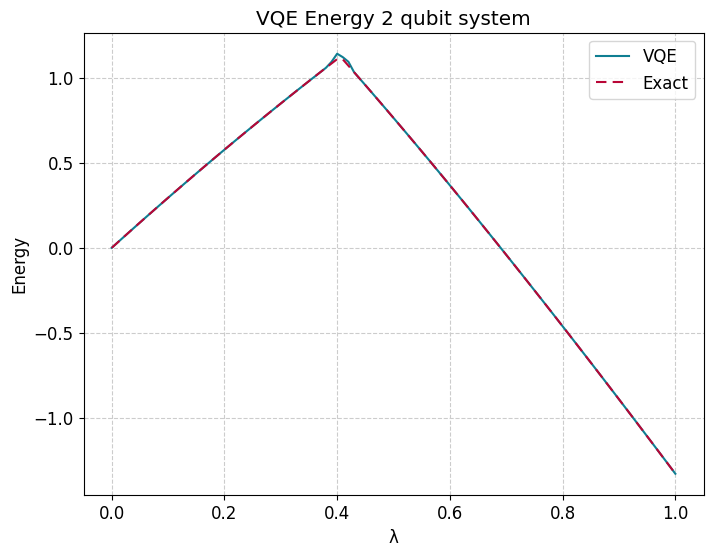
\includegraphics[scale=0.4]{VQE_2qubit.png}
        \end{center}

        \caption{The figure shows the VQE approximation of the ground state energy of the 2-qubit system, plotted against the exact ground state energy, as functions of the parameter \(λ\).}
        \label{fig:VQE2q}
\end{figure}
Figure \ref{fig:VQE2q} shows the VQE approximation of the ground state energy of the 2-qubit system, plotted against the exact ground state energy, as functions of the parameter \(λ\). This was again solved, using a gradient descent method to find the optimal parameters \(θ_1,θ_2,ϕ_1,ϕ_2\) The VQE method was successful in finding the ground state energy of the Hamiltonian, and the results are very close to the exact ground state energy. Even for a two qubit system, the VQE method seems to be a very effective and accurate method for finding the ground state energy of the Hamiltonian. \newline
We can see slight inaccuries at \(λ=0.4\). This is where the ground state has a crack in energy and starts to decrease. It is expected that this point would be the most difficult to approximate. \newline

\section{f)}
In this section, I will ecplore the Lipkin Hamiltonian for the \(3\times 3\) matrix with total spin \(J=1\), and the \(5 \times 5\) matrix with total spin \(J=2\). \newline
We start by defining the Hamiltonian in second quantization
\[
\begin{aligned}
        H_0 &= \frac{1}{2} ϵ ∑_{p σ}^{} σ a_{pσ}^{†} a_{pσ} \\
        H_1 &= -\frac{1}{2} V ∑_{pp'σ}^{} a_{σp+}^{†} a_{σp'}^{†} a_{σp'} a_{σp}\\
        H_2 &= -\frac{1}{2} W ∑_{pp'σ}^{} a_{σp+}^{†} a_{-σp'}^{†} a_{-σp'} a_{σp}  \\
        H &= H_0 + H_1 + H_2
\end{aligned}
\]
rewriting in terms of the quasispin operators, we get:
\[
\begin{aligned}
H_0 &= ϵ J_z \\
H_1 &= -\frac{V}{2} (J_+^2 + J_-^2) \\
H_2 &= -\frac{W}{2} (-N +J_+ J_- + J_- J_+)
\end{aligned}
\]
For both the \(J=1 \text{ and } J=5\), we set \(W=0\) so that \(H = H_0+H_1\).
We now want to show how the Hamiltonian will look in matrix representation. First we need to introduce how the quasispin operators act on a state. 
\[
\begin{aligned}
J_z \ket{j,m_j} &= m_j ℏ \ket{j,m_j} \\
J_± \ket{j,m_j} &= \sqrt{j(j+1) - m_j(m_j ± 1)} ℏ \ket{j,m_j ± 1}
\end{aligned}
\]
To convert the \(J=1\) Hamiltonian to matrix form, we can use \(\bra{1,-1},\bra{1,0} \bra{1,1}\) to represent the rows and \(\ket{1,-1},\ket{1,0},\ket{1,1}\) to represent the columns. First we will find the matrix elements we get from the \(J_z\) operator.
\[
J_z \rightarrow
\begin{pmatrix} 
  \bra{1,-1} J_z \ket{1,-1} & \bra{1,-1} J_z \ket{1,0} & \bra{1,-1} J_z \ket{1,1} \\
        \bra{1,0} J_z \ket{1,-1} & \bra{1,0} J_z \ket{1,0} & \bra{1,0} J_z \ket{1,1} \\
        \bra{1,1} J_z \ket{1,-1} & \bra{1,1} J_z \ket{1,0} & \bra{1,1} J_z \ket{1,1}
\end{pmatrix}   
\] 
Here we can see that only the diagonal elements are non-zero
\[
\begin{pmatrix}
  -ℏ & 0 & 0 \\
  0 & 0 & 0 \\
  0 & 0 & ℏ
\end{pmatrix}
\]
Now we can find the matrix elements we get from the \(J_±\) operator.
\[
\begin{aligned}
        J_+^2 &\rightarrow
        \begin{pmatrix}
          \bra{1,-1} J_+ ^2 \ket{1,-1} & \bra{1,-1} J_+ ^2 \ket{1,0} & \bra{1,-1} J_+ ^2 \ket{1,1} \\
                \bra{1,0} J_+ ^2 \ket{1,-1} & \bra{1,0} J_+ ^2 \ket{1,0} & \bra{1,0} J_+ ^2 \ket{1,1} \\
                \bra{1,1} J_+ ^2 \ket{1,-1} & \bra{1,1} J_+ ^2 \ket{1,0} & \bra{1,-1} J_+ ^2 \ket{1,1}
        \end{pmatrix}\\
        J_-^2 &\rightarrow
        \begin{pmatrix}
                \bra{1,-1} J_- ^2 \ket{1,-1} & \bra{1,-1} J_- ^2 \ket{1,0} & \bra{1,-1} J_- ^2 \ket{1,1} \\
                \bra{1,0} J_- ^2 \ket{1,-1} & \bra{1,0} J_- ^2 \ket{1,0} & \bra{1,0} J_- ^2 \ket{1,1} \\
                \bra{1,1} J_- ^2 \ket{1,-1} & \bra{1,1} J_- ^2 \ket{1,0} & \bra{1,-1} J_- ^2 \ket{1,1}
        \end{pmatrix} 
\end{aligned}
\]
The \(J_+^2\) operator only contributes to the top right element, and the \(J_-^2\) operator only contributes to the bottom left element. So we get
\[
\begin{aligned}
        J_+^2 &\rightarrow
        \begin{pmatrix}
          0 & 0 & 2ℏ \\
          0 & 0 & 0 \\
          0 & 0 & 0
        \end{pmatrix} \\
        J_-^2 &\rightarrow
        \begin{pmatrix}
          0 & 0 & 0 \\
          0 & 0 & 0 \\
          2ℏ & 0 & 0
        \end{pmatrix}
\end{aligned}
\]
Combining the results, we get the matrix representation of the Hamiltonian for the \(J=1\) system
\[
\begin{pmatrix}
  -ℏ & 0 & 2ℏ \\
  0 & 0 & 0 \\
  2ℏ & 0 & ℏ
\end{pmatrix}
\]
If we set \(ℏ = 1\), and since \(H_0 = ϵJ_z\) and \(H_1 = -\frac{V}{2}(J_+ ^2 + J_-^2)\) we get the folloing Hamiltonian matrix for the \(J=1\) system. 
\[
H_{J=1} = 
\begin{pmatrix}
  -ϵ & 0 & -V \\
  0 & 0 & 0 \\
  -V & 0 & ϵ
\end{pmatrix}
\]
For \(J=2\) we have a \(5 × 5\) matrix, which is given by:
\[
H_{J=2} = 
\begin{pmatrix}
  -2ϵ & 0 & \sqrt{6}V & 0 & 0 \\
        0 & -ϵ + 3W & 0 & 3V & 0 \\
        \sqrt{6}V & 0 & 4W & 0 & \sqrt{6}V \\
        0 & 3V & 0 & -ϵ + 3W & 0 \\
        0 & 0 & \sqrt{6}V & 0 & -2ϵ
\end{pmatrix}
\]
Now we want to show how these two Hamiltonian can be rewritten in terms of Pauli spin matrices. \newline
Lets start with the \(J=1\) case. First, lets recall the Pauli matrices
\[
\begin{aligned}
σ_x &= \begin{pmatrix}
        0 & 1 \\
        1 & 0
\end{pmatrix} \\
σ_y &= \begin{pmatrix}
        0 & -i \\
        i & 0
\end{pmatrix} \\
σ_z &= \begin{pmatrix}
        1 & 0 \\
        0 & -1
\end{pmatrix}
\end{aligned}
\]
To form the \(J=1\) Hamiltonian in terms of the Pauli matrices, I will start by identifying the diagonal elements. 
\[
\begin{aligned}
σ_z ⊗ I &= 
\begin{pmatrix}
  1&0\\0&-1
\end{pmatrix}
⊗
\begin{pmatrix}
  1&0\\0&1
\end{pmatrix}
\\
&= 
\begin{pmatrix}
        1&0&0&0\\
        0&1&0&0\\
        0&0&-1&0\\
        0&0&0&-1
\end{pmatrix}\\
σ_z ⊗ σ_z &=
\begin{pmatrix}
        1&0\\0&-1
\end{pmatrix}
⊗
\begin{pmatrix}
        1&0\\0&-1
\end{pmatrix}\\
&=
\begin{pmatrix}
        1&0&0&0\\
        0&-1&0&0\\
        0&0&-1&0\\
        0&0&0&1
\end{pmatrix}
\end{aligned}
\]
Adding these matrices together and including a factor of \(-
\frac{ϵ}{2}\)
\[
H_0 = -\frac{ϵ}{2} (σ_z ⊗ I + σ_z ⊗ σ_z)\\
=
\begin{pmatrix}
        -ϵ&0&0&0\\
        0& 0&0&0\\
        0&0&ϵ&0\\
        0&0&0&0
\end{pmatrix}
\]
Now we need to find a combination of Pauli spin matrices for the anti-diagonal elements in the \(3 \times 3\) matrix. 
\[
\begin{aligned}
σ_x ⊗ I &= 
\begin{pmatrix}
  0&1\\1&0
\end{pmatrix}
⊗
\begin{pmatrix}
  1&0\\0&1
\end{pmatrix}
\\
&= 
\begin{pmatrix}
        0&0&1&0\\
        0&0&0&1\\
        1&0&0&0\\
        0&1&0&0
\end{pmatrix}\\
σ_x ⊗ σ_z &=
\begin{pmatrix}
        0&1\\1&0
\end{pmatrix}
⊗
\begin{pmatrix}
        1&0\\0&-1
\end{pmatrix}\\
&=
\begin{pmatrix}
        0&0&1&0\\
        0&0&0&-1\\
        1&0&0&0\\
        0&-1&0&0
\end{pmatrix}
\end{aligned}
\]
Adding these together with a factor of \(-\frac{V}{2}\), we get
\[
H_1 = -\frac{V}{2} (σ_x ⊗ I + σ_x ⊗ σ_z) \\
= 
\begin{pmatrix}
        0&0&-V&0\\
        0& 0&0&0\\
        -V&0&0&0\\
        0&0&0&0
\end{pmatrix}
\]
From this, the total \(J=1\) Hamiltonian is
\[
H_{J=1} = 
\begin{pmatrix}
        -ϵ&0&-V&0\\
        0& 0&0&0\\
        -V&0&ϵ&0\\
        0&0&0&0
\end{pmatrix}
\]
In order to find an expression for the \(J=2\) Hamiltonina with Pauli matrices, I will have to use block diagonalization to simplify the problem. The thought is to separate the \(5 \times 5\) Hamiltonian into two pieces, one \(3 \times 3\) and one \(2\times 2\). The \(3 \ times 3\) will hold the even numbered column, while the \(2 \times 2\) will hold the odd numbered columns. 

\[
\begin{aligned}
H_{3 \times 3} &= 
\begin{pmatrix}
  -2ϵ & \sqrt{6}V & 0\\
  \sqrt{6}V & 0 & \sqrt{6}V\\
  0& \sqrt{6}V&2ϵ
\end{pmatrix} \\
H_{2 \times 2} &= 
\begin{pmatrix}
  -ϵ & 3V \\
  3V & ϵ
\end{pmatrix}
\end{aligned}
\]
Combining these will look like:
\[
H = 
\begin{pmatrix}
  H_{3× 3} & \\
  & H_{2× 2}
\end{pmatrix}
\]
Whats nice about this method, is that the collected eigenvalues of each blocks (\(H_{3\times 3} \text{ and } H_{2× 2} \) ) will have the same eigenvalues as the total \(H_{J=2}\) Hamiltonian. So lets now focus on identifying each blocks with Pauli matrices.\newline
Lets start with the \(H_{3\times 3}\):
\[
H_{3× 3} = -ϵ(σ_z⊗ I + σ_z \otimes σ_z) + \frac{V}{2} \sqrt{6} (I ⊗ σ_x + σ_z⊗ σ_x + σ_x⊗ σ_x +σ_y⊗ σ_y  ) 
\]
This will give us the desired \(H_{3\times 3}\) matrix. For the \(H_{2 \times 2}\) we get

\[
H_{2× 2} = -ϵ σ_z +3V σ_x
\]
Notice that the \(H_{3\times 3}\) is actually a \(4\times 4\), but the last rows and columns are \(0\)'s. \newline
Figure \ref{fig:PauliFigs} shows two plots. The left figure shows the eigenvalues of the \(J=1\) Hamiltonian, and the right hand figure shows the eigenvalues of the \(J=2\) Hamiltonian. The eigenvalues are functions of an interraction parameter \(V\). \newline
In figure \ref{fig:PauliFigs} we can see a pattern in both figures. The left hand figure displays the eigenvalues of the \(J=1\) Hamiltonian and the right hand figure shows the eigenvalues of the \(J=2\) Hamiltonian. We have, as expected, 3 and 5 eigenvalues for each Hamiltonian. We can see how when the interraction paramter \(V\) increases, the eigenvalues diverge. This is expected as interraction strength increases. 

\begin{figure}[h]
        \begin{center}
                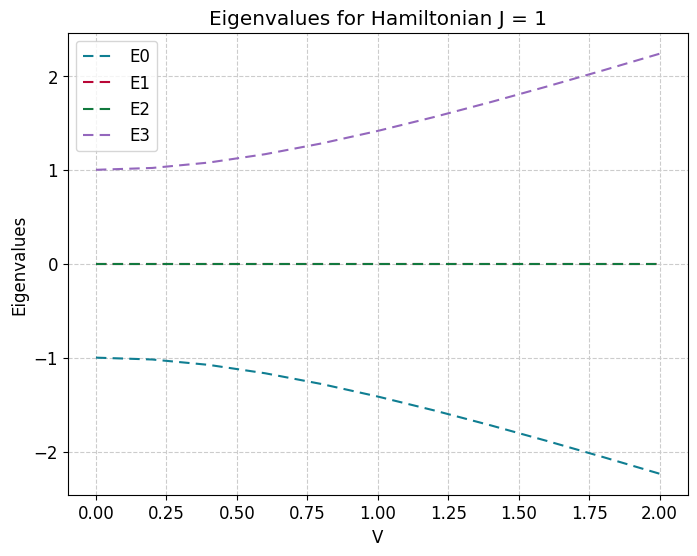
\includegraphics[scale=0.3]{J1Hamil.png}
                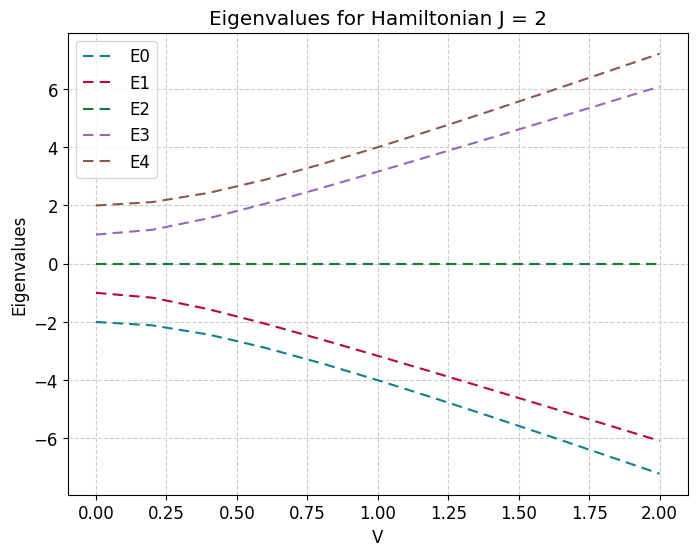
\includegraphics[scale=0.3]{J2Hamil.png}       
        \end{center}
        \caption{The left figure shows the eigenvalues of the \(J=1\) Hamiltonian, and the right hand figure shows the eigenvalues of the \(J=2\) Hamiltonian.}
        \label{fig:PauliFigs}
\end{figure}\newpage


\section{g)}
The ansatzes used for these approximations were as follows:
\[
\begin{aligned}
\ket{ψ_{J=1}} &= CNOT ⋅  R_y(ϕ) ⊗ I ⋅CNOT ⋅  I ⊗ R_x(θ) \ket{00} \\
\ket{ψ_{J=2}} &= R_y(ϕ_1) ⊗ R_y(ϕ_2) ⊗ R_y(ϕ_3) ⋅ CNOT ⊗ I ⋅ I ⊗ CNOT ⋅  R_y(ϕ_4) ⊗ R_y(ϕ_5) ⊗ R_y(ϕ_6) \ket{000}
\end{aligned}
\]
\begin{figure}
        \begin{center}
                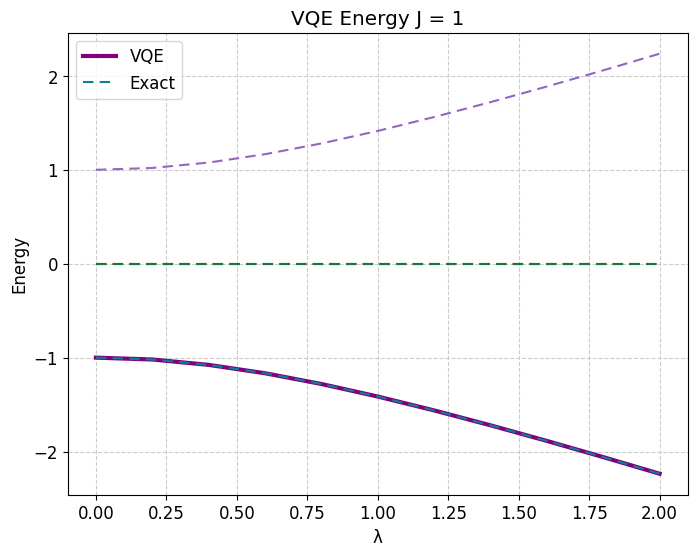
\includegraphics[scale=0.3]{VQEj1.png}
                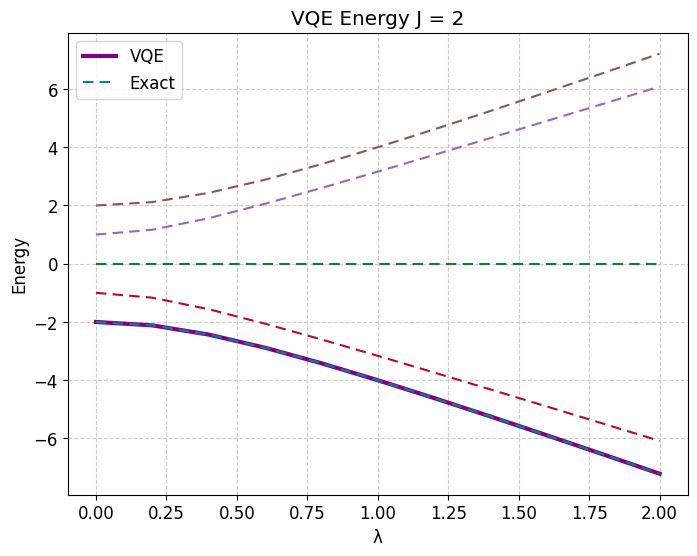
\includegraphics[scale=0.3]{VQEj2.png}       
        \end{center}
        \caption{The left figure shows the VQE method for the \(J=1\) Hamiltonian, and the right hand figure shows the VQE method for the \(J=2\) Hamiltonian.}

        \label{fig:PauliVQE}
\end{figure}
Figure \ref{fig:PauliVQE} shows the VQE method for each of the Hamiltonians. We can see that the gradient descent method still does a very good job at approximating the ground state energy of the system. The approximation is almost perfectly aligned with the true ground state we obtained from diagonalization. 



\section{Code}
\href{https://github.com/hishemok/FYS5419/tree/master/Project_1}{github.com/hishemok/FYS5419/tree/master/Project\_1}

\section{VQE measurements}
The measurements I did when I did the VQE method, was to always construct the Hamiltonian with Pauli matrices. This was done to recreate the methods used experimentally. But this meant, that to measure a qubit's state, we could not just take the energy expectation value, but rather we had to measure on each Pauli matrix. Following is a table of Pauli measurements, and the operator \(U\) we had to use to measure the qubit. 
\begin{table}[h]
        \centering
        \begin{tabular}{c|c}
            \textbf{Pauli Measurement} & \textbf{Operator U} \\ \hline
            $Z \otimes I$ & $I \otimes I$ \\
            $X \otimes I$ & $H \otimes I$ \\
            $Y \otimes I$ & $H S^\dagger \otimes I$ \\
            $I \otimes Z$ & $(I \otimes I) \text{ SWAP}$ \\
            $I \otimes X$ & $(H \otimes I) \text{ SWAP}$ \\
            $I \otimes Y$ & $(H S^\dagger \otimes I) \text{ SWAP}$ \\
            $Z \otimes Z$ & $CX_{1,0}$ \\
            $X \otimes Z$ & $CX_{1,0} (H \otimes I)$ \\
            $Y \otimes Z$ & $CX_{1,0} (H S^\dagger \otimes I)$ \\
            $Z \otimes X$ & $CX_{1,0} (I \otimes H)$ \\
            $X \otimes X$ & $CX_{1,0} (H \otimes H)$ \\
            $Y \otimes X$ & $CX_{1,0} (H S^\dagger \otimes H)$ \\
            $Z \otimes Y$ & $CX_{1,0} (I \otimes H S^\dagger)$ \\
            $X \otimes Y$ & $CX_{1,0} (H \otimes H S^\dagger)$ \\
            $Y \otimes Y$ & $CX_{1,0} (H S^\dagger \otimes H S^\dagger)$ \\
        \end{tabular}
        \caption{Pauli measurement operators with no identity.}
    \end{table}
    

\end{document}











